% adapté de la RIG version française

\documentclass[french]{./sageo}

\confShortName{SAGEO'2017}
\confLongName{SAGEO'2017 - Rouen, 6-9 novembre 2017}

\usepackage[utf8]{inputenc} 
\usepackage[T1]{fontenc}
\usepackage{lmodern}
\usepackage{textcomp}
\usepackage{amsmath}
\usepackage{graphicx}
\usepackage{multirow}
\usepackage[noend]{algorithmic}
\usepackage[linesnumbered,ruled,vlined,boxed,commentsnumbered]{algorithm2e}

\firstpagenumber{1}

% \title[short header title]{title}
\title{Titre de l'article}

\author[1]{Prénom1}{Nom1}
\author[2]{Prénom2}{Nom2}

% addresses are automatically numbered
\address{adresse1}
        {name1@email}
 \address{adresse2}
        {name2@email}       

\resume{Résumé.}

\motscles{Quelques mots clés}

\keywords{En anglais}

\abstract{Abstract in English}

\begin{document}

\maketitle

\newpage

\section{Introduction}

\section{Section 1}

\subsection{Sous-section 1}

\subsubsection{Sous-sous-section 1}

\begin{figure*}[h]
   \centering  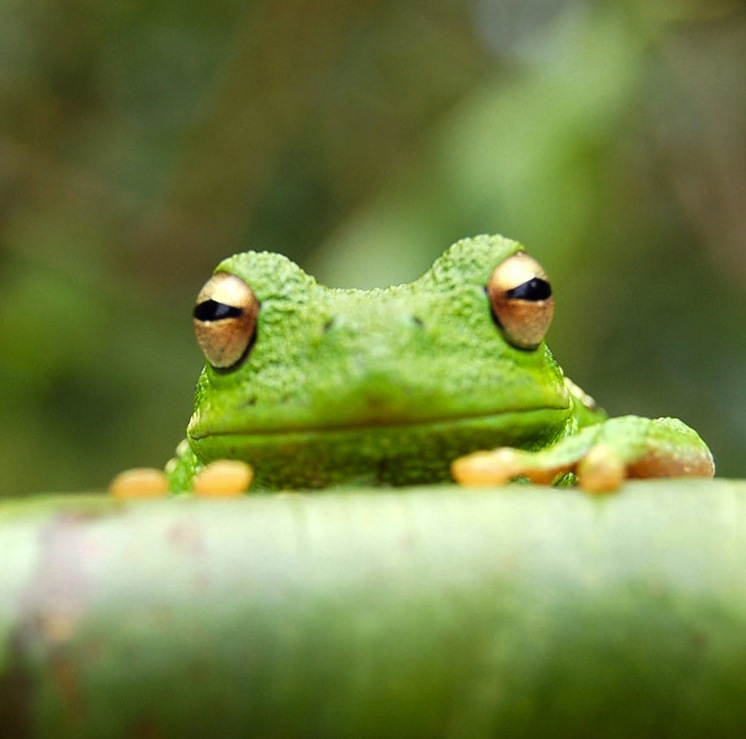
\includegraphics[width=8cm]{grenouille.jpg}
  \caption{\label{fig:1} Une grenouille bien verte.}
\end{figure*}

\subsection{Sous-section 2}

\section{Section 2}

Listes :
\begin{itemize}
\item ligne 1 (cf. équation \ref{eq:form1})
\item ligne 2 (cf. équation \ref{eq:form2})
\end{itemize}

Formules :

\begin{equation}
	R = \frac{d_1}{d_2}
	\label{eq:form1}
\end{equation}

\begin{equation}
	\sin(\alpha) = \frac{h}{l}
    \label{eq:form2}
\end{equation}

\begin{table*}[h!]
\begin{center}
\caption{\label{tab:1} Exemple de tableau}
 \scriptsize
      \begin{tabular}{|c|c|c|c|c|}
   \hline
   \multirow{2}*{ Clients} & \multicolumn{2}{| c |}{Départ }  & \multicolumn{2}{| c |}{ Arrivée}\\
   \cline{2-5}
      & Station  & Période de Temps & Station  & Période de Temps \\\hline
   client 1 (c1) & 3  & 2 & 1 & 4 \\\hline
   client 2 (c2)   &   2  & 2 & 3 & 3\\\hline
   client 3 (c3)   &   2 & 2 & 3 & 4  \\\hline
   client 4 (c4)   &   3 & 2 & 2 & 3  \\\hline
   client 5 (c5)   &   3 & 2 & 2 & 4  \\\hline
  client 6 (c6)   &   2  & 4 & 3 & 5\\\hline
   client 7 (c7)   &   3  & 3 & 2 & 6  \\\hline
   client 8 (c8)   &   1 & 5 & 3 & 6 \\\hline
   client 9 (c9) & 2  & 6 & 3 & 7 \\\hline
    client 10 (c10)  &   3 & 7 & 1 & 9 \\\hline
   client 11 (c11) & 1  & 6 & 2 & 7 \\\hline
%\hline
\end{tabular}
\end{center}
\end{table*}

Exemple d'algorithme :

\begin{algorithm}[h!]
\label {algo}
 \KwData{
 $G(V,A,C,R,U)$ \; \tcc{commentaire}}
 \KwResult{
 $Paths_{Cars}, \; Relocation,\; SatisfiedDemands, Paths_{Agents}  $
 }
 initialization\;
 $Paths_{Agents} \gets \emptyset $ /* l'ensemble de chemins... */ \;
 $j \gets 1$ \;
 $costPath_j  \gets 0$ \;
 \While { $ (j \le  nb_{Veh}) \wedge (costPath_j \leq 0)  $ }
 {
 $ path_j \gets Dijkstra(G(V,A, C,R)) $ \;
$ costPath_j \gets  Cost (path_j)$ \;
  \ForAll { $(v^{k}_{t'},v^{i}_{t}) \in path   $}
{
 \ForAll {$ U_{r^{i}_{t'',t''+1}} $  }
 {....
 }
$ Paths_{Cars} \gets Paths_{Cars} \cup path_j $  \;
 }
$j \gets j+1$ \;
 }
$Paths_{Agents} \gets  routeAgents (Relocation ); $
 \caption{un algorithme très glouton}
\end{algorithm}

\section{Conclusion}

Blabla \cite{newton}, mais aussi \cite{castel} et encore \cite{Ada2007,and06,adh12} \footnote{Ces travaux s'inscrivent...}.

\bibliography{sageo-ref}

\end{document}